
\documentclass[a4paper,12pt]{article}
\usepackage[margin=1in]{geometry}

\usepackage[T2A]{fontenc}			% кодировка
\usepackage[utf8]{inputenc}			% кодировка исходного текста
\usepackage[english,russian]{babel}	% локализация и переносы
\usepackage{graphicx}                % Математика
\usepackage{amsmath,amsfonts,amssymb,amsthm,mathtools} 
\usepackage[T2A]{fontenc}
\usepackage[utf8]{inputenc}
\usepackage{color, colortbl}
\usepackage{wasysym}
\usepackage[warn]{mathtext}
%Заговолок
\author{Бичина Марина 
группа Б04-005 1 курса ФЭФМ}
\title{Лабораторная работа №1.3.3 \\ Измерение вязкости воздуха по течению в тонких трубках}
\date{\today}


\begin{document} % начало документа
\renewcommand{\labelenumii}{\arabic{enumii})}
\definecolor{strongRed}{RGB}{230,170,150}
\newcolumntype{g}{>{\columncolor{strongRed}}c}

\maketitle
\newpage

\section{Аннотация}

\paragraph{Цель работы:} 
\begin{enumerate}
\itemsep0em
\item 
экспериментально исследовать свойства течения газов по тонким трубкам при различных числах Рейнольдса
\item 
 выявить область применимости закона Пуазейля и с его помощью определить коэффициент вязкости воздуха 
\end{enumerate}
\paragraph{Оборудование:}
\begin{enumerate}
\itemsep0em
\item 
система подачи воздуха (компрессор, проводящие трубки)
\item
газовый счетчик барабанного типа
\item
спиртовой микроманометр с регулируемым наклоном
\item
 набор трубок различного диаметра с выходами для подсоединения микроманометра
\item
  секундомер
\end{enumerate}
\section{Теоретическая часть:}
\paragraph{}
Характер течения в трубе может быть ламинарным либо турбулентным. Для определения характера течения пользуются безразмерной величиной -- числом Рейнольдса:
\[
Re = \frac{\rho ua}{\eta}
\]
где 
\begin{enumerate}
\itemsep0em
\item 
$\rho$ -- плотность среды 
\item
$u$ -- характерная скорость потока
\item 
$\eta$ -- коэффициент вязкости среды
\item 
$a$ -- характерный размер системы 
\end{enumerate}
При достаточно малых значениях числа Рейнольдса, движение является ламинарным. После достижения некоторого критического значения, характер движения изменяется на турбулентный. В гладких трубах круглого сечения переход от ламинарного движения к турбулентному происходит при $Re \approx 10^3$\\
Для ламинарного движения объем газа $V$, протекающий за время $t$ по трубе длиной $l$, можно рассчитать по формуле Пуазейля:
\begin{equation}
Q_v = \frac{\pi r^4}{8l \eta}(P_1-P_2)
\end{equation}
Величина $Q_v$ -- называется расходом. Формула (1) позволяет определить вязкость жидкости по расходу.
\subsection{Описание установки:}
\begin{figure}
\centering
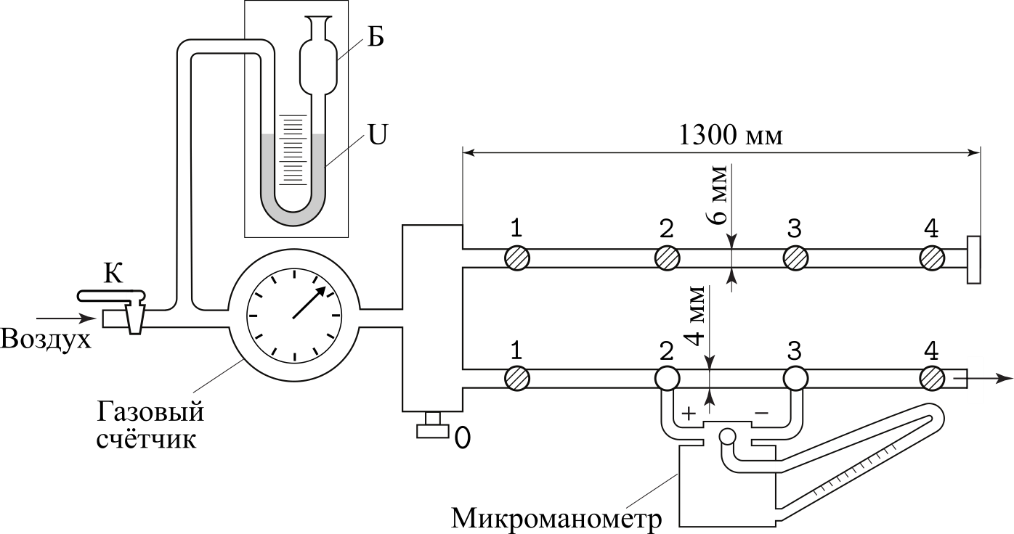
\includegraphics[width=0.7\linewidth]{setup.png}
\label{fig:setup}
\caption{Экспериментальная установка}
\end{figure}
\paragraph{Данные установки:}
\begin{enumerate}
\itemsep0em
\item
\textbf{Диаметры труб:}
\[d_1 = 3.90 \pm 0.05 \text{мм}\]
\[d_2 = 5.25 \pm 0.05 \text{мм}\]
\[d_3 = 3.00 \pm 0.10 \text{мм}\]
\item 
\textbf{Коэффициент для перевода давления в Па:}
\[k =  C \cdot \dfrac{\gamma_{\text{спирт залитый}}}{\gamma_{\text{спирт приборный}}}\cdot K \cdot 9.81 = 1.96\]
\item\textbf{ Расстояния между разъёмами на трубах:}
	\[
		l_1 = 50 \pm 0.1 \; \text{см},	\;\;\;\;\;\;\;\;\;\;\; l_2 = 40 \pm 0.1 \; \text{см},
	\]\[
		l_3 = 30 \pm 0.1 \; \text{см}, \;\;\;\;\;\;\;\;\;\;\; l_4 = 11 \pm 0.1 \; \text{см}.	
	\]
\end{enumerate}
\paragraph{}
Через кран К в экспериментальную установку попадает газ под давлением чуть более высоким, чем атмосферное.
За краном К установлен U-образный манометр показывающий разницу в давлении между входящим воздухом и атмосферой. 
Если давление в установке поднимается выше допустимого вода в манометре поднимается в баллон Б, который издаёт звук оповещающий экспериментатора.
Далее воздух проходим через газовый счётчик, измеряющий объём прошедшего через него газа.
После этого газ проходит через одну из двух трубок с заглушками, к которым можно подключать концы микроманометра.
\paragraph{}

\subsection{Контрольные вопросы:}
\begin{enumerate}
\itemsep0em
\item Что такое коэффициент вязкости? Сформулируйте закон Ньютона для вязкого трения и укажите границы его применимости в газах. \\\\ 
Силы вязкого (<<внутреннего>>) трения возникают между соседними слоями жидкости при ее движении, а также со стороны стенок трубы. Описываются они с помощью закона Ньютона:
\begin{equation}
\tau_{xy} = -\eta \frac{dv_{x}}{dy}
\end{equation}
где:
\begin{enumerate}
\itemsep0em
\item $\tau_{xy}$ -- касательное напряжение
\item $v_{x}$ -- скорость течения вдоль оси х
\item y -- координата y  
\item $\eta$ --вязкость; \\
$\eta \sim \frac{1}{3}\rho \overline{v} \lambda$ -- для идеального газа ($\lambda$ -- длина свободного пробега молекул газа относительно столкновений друг с другом)
\end{enumerate}
\item Что такое число Рейнольдса? Покажите, что число Рейнольдса есть отношение кинетической энергии жидкости к работе сил трения в единице объёма.\\\\
Безразмерная величина, показывающая характер течения жидкости -- число Рейнольдса:
\[
Re = \frac{\rho ua}{\eta}
\]

\item 
Опишите основные характеристики течения Пуазейля. Как меняется давление
вдоль трубы? Как меняется скорость течения в сечении трубы? Каково отношение
средней и максимальной скоростей течения?\\\\
Течение Пуазеля работает только для ламинарных потоков. Давление в трубе является линейно убывающей функцией координаты: 
\[P(x) = P_0 - \frac{\Delta P}{l}x\]
Средняя скорость вдвое меньше максимальной, имеет место параболическое распределение скоростей. 
\item 
Перечислите условия применимости формулы Пуазейля. С какой точностью эти
условия выполняются в вашем опыте?\\\\
Для применения формулы Пуазейля, необходимо иметь:
\begin{enumerate}
\item трубу с гладкими стенками
\item малость чисел Рейнольдса
\item условие несжимаемости газа
\end{enumerate} 
Гладкость обеспечивается малостью диаметра трубки по сравнению с ее длиной. Малость чисел Рейнольдса мы можем обеспечить, выполняя задание не выходя за рамки критического значения $Re \approx 10^3$. Условие несжимаемости рассмотрено ниже
\item 
С какой точностью течение газа в условиях опыта можно считать несжимаемым?
Вычислите максимальное число Маха (отношение скорости течения к скорости звука) в условиях опыта\\\\
Максимальное $\Delta P$ полученное на опыте $\Delta P_\text{max} \approx 310$ Па. При этом атмосферное давление $P_0 = 10^5$ Па, то есть $\Delta P / P \sim 10^{-3}$, из-за чего можно считать, что газ практически не сжимается.

Максимальную скорость можно оценить как $u_\text{max} = 2 \langle u \rangle = Q / (\pi R^2)$. $Q_\text{max} \approx 0.12 $ л/с, найдём $u_\text{max} = 0.12 \cdot 10 ^ {-3} / (\pi \cdot 0.0039 ^ 2) = 2.5$ м/с. Максимальное число маха $M_\text{max} = u_\text{max} / c = 2.5 / 340 \sim 0.01 $.
\item
Что такое ламинарное и турбулентное течение? При каких условиях течение может стать турбулентным? Как переход к турбулентности можно обнаружить на опыте?\\\\
При ламинарном движении поле скоростей образует набор непрерывных линий тока, а слои жидкости не перемешиваются между собой. Давление на манометре в таком случае постоянно.\\
При турбулентном движении образуются вихри, активно перемешиваются слои. В таком случае на манометре можно увидеть заметные колебания, поскольку существуют существенные флуктуации скорости течения и давления.\\
Переход к турбулентности происходит после некоторого увеличения расхода газа, поскольку вместе с этим возрастает число Рейнольдса (происходит увеличение сверх критического значения)
\item 
По экспериментальному значению коэффициента вязкости оцените размеры молекул воздуха\\
Возьмём $\eta = 1.7 \cdot 10^{-5}$ Па $\cdot$ с:

\[
\eta \sim \frac{1}{3}\rho \bar{v} \lambda = \frac{1}{3} \rho \sqrt{\frac{3 R T}{\mu}} \frac{1}{n \sigma} = \frac{1}{3} \rho \sqrt{\frac{3 R T}{\mu}} \frac{\mu}{N_a \rho \sigma} = \frac{1}{3} \frac{\sqrt{3 R T \mu}}{N_a \sigma} ,
\]\[
\sigma = \frac{1}{3} \frac{\sqrt{3 R T \mu}}{N_a \eta} = \frac{1}{3} \frac{\sqrt{3 \cdot 8.314 \cdot 300 \cdot 0.029}}{6 \cdot 10^{23} \cdot 1.7 \cdot 10^{-5}} = 4.8 \cdot 10^{-19} \text{м}^2 = 48 \; \mathring{A}^2,
\]\[
r = \sqrt{\frac{\sigma}{\pi}} = \sqrt{\frac{48}{\pi}} \approx 4 \; \mathring{A}.
\]

\item 
Как вязкость газа зависит от его температуры и давления? Оцените погрешность
измерения коэффициента вязкости в вашем опыте, обусловленную неопределенностью в параметрах окружающей среды (температура, давление, влажность)\\
Из п7 имеем зависимость вязкости от температуры как $\eta \sim sqrt{T}$
\item
Какие независимые безразмерные комбинации можно составить из параметров задачи о течении несжимаемой жидкости по прямой трубе? Каков, согласно теории
размерностей, общий вид зависимости расхода от перепада давления $Q(\Delta P)$?\\\\
Из параметров задачи о течении несжимаемой жидкости по прямой трубе можно составить 2 независимые безразмерные комбинации: число Рейнольдса и некоторую функцию $\psi = \dfrac{R\Delta P}{l \rho u^2}$ где  $\psi$ -- это отношение перепада давления в трубе к скоростному напору.
    
    Общий вид зависимости расхода от перепада давления $Q(\Delta P)$ при ламинарном режиме: $$Q = const \cdot \frac{R^{4}}{\eta} \cdot \frac{\Delta P}{l}$$
\item Пользуясь методом размерностей,рассмотрите задачу о силе сопротивления, действующей на шарик радиусом $r$, обтекаемый потоком несжимаемой жидкости со скоростью $u$, имеющей плотность $\rho$ и вязкость $\eta$ . Покажите, что 1) если сила прямо пропорциональна скорости, то имеет место закон Стокса $F \sim \eta u r $,2) если сила со-противления не зависит от вязкости, то зависимость имеет вид $F \sim \rho u^2 r^2 $. 

1) $F = \left[ \dfrac{\text{кг} \cdot \text{м}}{\text{с} ^ 2} \right], \; \eta = \left[ \dfrac{\text{кг}}{\text{м} \cdot \text{с}} \right], \; u = \left[ \dfrac{\text{м}}{\text{с}} \right], \; r = [\text{м}] \rightarrow F = \left[ \dfrac{\text{кг}}{\text{м} \cdot \text{с}} \cdot \dfrac{\text{м}}{\text{с}} \cdot \text{м} \right] = \eta u r $ 

2) $F = \left[ \dfrac{\text{кг} \cdot \text{м}}{\text{с} ^ 2} \right], \; \rho = \left[ \dfrac{\text{кг}}{\text{м} ^ 3} \right], \; u = \left[ \dfrac{\text{м}}{\text{с}} \right], \; r = [\text{м}] \rightarrow F = \left[ \dfrac{\text{м} ^ 2}{\text{с} ^ 2} \cdot \dfrac{\text{кг}}{\text{м} ^ 3} \cdot \text{м} ^ 2 \right] = u^2 r^2 \rho $

\end{enumerate}
\section{Ход работы:}
\begin{enumerate}
\renewcommand{\labelenumii}{\arabic{enumii})}
\itemsep0em
\item Подготовим установку к работе:
\item Проведём предварительный запуск установки и убедимся в её работоспособности:
	\begin{enumerate}
	\item Подсоединим манометр к двум соседним выводам на конце одной из трубок 				(рекомендуется начать с трубки диаметром $d \approx 4$ мм). Убедимся, что все отверстия, кроме одного -- выходного -- плотно завинчены пробками.
	\item Убедимся, что кран К, соединяющий компрессор с установкой, закрыт. Включим компрессор. Переведите рычажок микроманометра в рабочее положение (+).
	\item Медленно приоткрывая кран К и непрерывно контролируя показания микроманометра, создадим небольшой поток воздуха через трубку. 
	\item Пронаблюдаем за показаниями приборов в зависимости от интенсивности потока  через  трубку.  Убедимся в том,  что  при  неизменном  положении крана К показания манометра стабильны, а стрелка расходомера вращается равномерно.
	\end{enumerate}
	
\item Проведем предварительные расчёты:
	\begin{enumerate}
	\item Рассчитаем значение расхода $Q_{\text{кр}}$, при котором число Рейнольдса в трубке станет равным критическому $Re_{\text{кр}} \approx 10^3$. Для предварительной оценки прими вязкость воздуха равной $\eta_\text{возд} \approx 2 \cdot 10^{-5}$ Па $\cdot$ с, плотность воздуха определим по уравнению идеального газа. В качестве характерной скорости  потока используем её  среднее  значение $\bar{u} = Q/ \pi R^2$.
\[
Re = \frac{\rho \bar{u} a}{\eta} = \frac{\rho Qa}{\pi R^2 \eta}
\]
\[
Q = \frac{Re \pi R \eta}{\rho} = \frac{10^3 \cdot 3.14 \cdot 2 \cdot 10^{-3} \cdot 2 \cdot 10^{-5}}{2 \cdot 10^{-5}} \approx 10^{-4}\dfrac{\text{мл}^3}{\text{c}} = 0.1 
\dfrac{\text{л}^3}{\text{c}}
\]
\end{enumerate}
\item
Найдем вязкость воздуха для трубки диаметром $d = 3.90 \pm 0.05$ мм: \\
На основании экспериментально полученных данных построим таблицу 1. Выделенное значение соответствует давлению, при котором характер движения воздуха был изменен на турбулентное:
\begin{table}[h]
\setlength{\tabcolsep}{2pt}
\begin{tabular}{|c||c|c|c|c|c|c|c|g|c|c|c|c|}
\hline 
$\Delta P$, Па & 18 & 37 & 59 & 78 & 98 & 118 & 139 & 157 & 196 & 235 & 274 & 314 \\ 
\hline 
$Q \cdot 10^{-3}$ л/с & 11.46 & 22.84 & 35.96 & 47.50 & 59.27 & 69.34 & 80.50 & 87.16 & 94.36 & 102.03 & 109.16 & 115.66 \\ 
\hline 
\end{tabular} 
\caption{Значения показаний, снятых с установки}
\end{table}
\item
По полученным данным \textbf{построим график зависимости $\Delta P(Q)$, воспользовавшись методом наименьших квадратов} $y=a+bx$:
\begin{equation}
b = \frac{\langle xy \rangle - \langle x \rangle \langle y \rangle}{\langle x^2 \rangle - \langle x \rangle^2} \;\;\;\;\;\;
b = \frac{\langle Q \Delta P \rangle - \langle Q \rangle \langle \Delta P \rangle}{\langle Q^2 \rangle - \langle Q \rangle^2} \;\;
\label{mnk}
\end{equation}
Погрешность в этом случае можно найти по формуле: 
\begin{equation}
\sigma_b \approx \frac{1}{\sqrt{N}}\sqrt{\frac{\langle \Delta P ^2 \rangle - \langle \Delta P \rangle ^ 2}{\langle Q^2 \rangle - \langle Q \rangle ^ 2} - b^2} 
\end{equation}
\begin{tabular}{|c|c|c|c|c|}
\hline 
$\langle Q \rangle$ & $\langle \Delta P \rangle$ & $\langle Q \cdot \Delta P \rangle$ & $\langle Q^2 \rangle$ & $\langle \Delta P^2 \rangle$ \\ 
\hline 
46.7 $\cdot 10^{-3}$ & 78.14 & 4579.8 $\cdot 10^{-3}$ & 2714.8 $\cdot 10^{-6}$ & 7729.6 \\ 
\hline 
\end{tabular} 
\[b = \frac{4579.8 \cdot 10^{-3} - 46.7 \cdot 10^{-3} \cdot 78.14}{2714 \cdot 10^{-6} - (46.7 \cdot 10^{-3})^2} = 1.7 \cdot 10^3 \]\;\;\;\; \[\sigma_{b} = \frac{1}{\sqrt{7}}\sqrt{\frac{7729.6 - 78.14^2}{2714 \cdot 10^{-6} - (46.7 \cdot 10^{-3})^2}} = 0.66 \cdot 10^3\]
\begin{center}
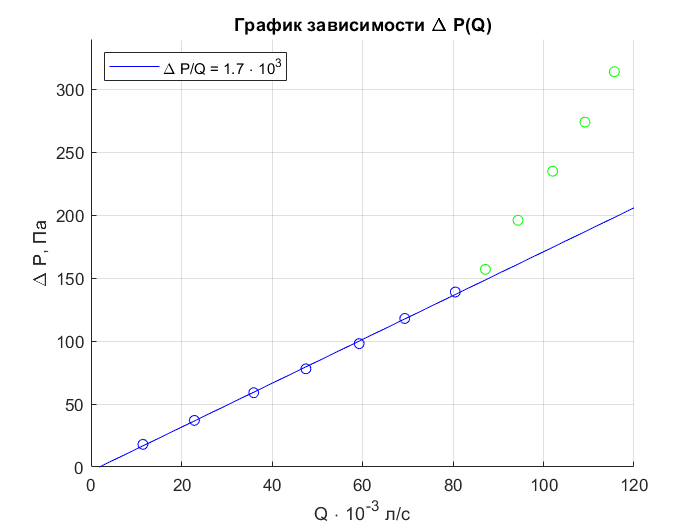
\includegraphics[width=0.9\linewidth]{plot_1.png}
\end{center}
Выразим $\eta$ из формулы Пуазейля и подставим значения:
\[
\eta = \dfrac{\pi R^4}{8 l} \dfrac{\Delta P}{Q} = \dfrac{\pi \cdot 0.0039 ^ 4}{8 \cdot 2^4 \cdot 0.5 \cdot 0.55 \cdot 10^{-6}} = 2.06 \cdot 10^{-5} \text{Па} \cdot \text{с},
\]
\[
\sigma_\eta = \eta \cdot \sqrt{4 \cdot \left( \frac{\sigma_R}{R} \right) ^ 2 + \left( \frac{\sigma_l}{l} \right) ^ 2 + \left( \frac{\sigma_b}{b} \right) ^ 2}, 
\]\[
\sigma_\eta = 2.06 \cdot 10^{-5} \cdot \sqrt{4 \cdot \left(\frac{0.05}{3.9} \right) ^ 2 + \left( \frac{0.1}{50} \right) ^ 2 + \left( \frac{0.01}{0.55} \right) ^ 2} = 0.07 \cdot 10 ^ {-5}.
\]

Получили $\eta = (2.06 \pm 0.07) \cdot 10^{-5}$ Па $\cdot$ с.\\
Далее рассчитаем критическое число Рейнольдса для воздуха, учитывая, что турбулентности начались при $Q = 0.09$ л/с:

\[
Re_\text{кр} = \frac{\rho \langle u \rangle d}{\eta} = \frac{4 Q \rho d}{\eta \pi d^2} = \frac{4 Q \rho}{\eta \pi d} = \frac{4 \cdot 0.09 \cdot 10^{-3} \cdot 1.2}{2.06 \cdot 10^{-5} \cdot \pi \cdot 0.0039} \approx 1700
\] 
\item Найдем вязкость воздуха для трубки диаметром $d = 5.25 \pm 0.05$ мм: \\
Занесем в таблицу 2 данные, полученные в эксперименте для трубы  $d = 5.25 \pm 0.05$ мм.
\begin{table}[h]
\begin{center}
\setlength{\tabcolsep}{2pt}
\begin{tabular}{|c||c|c|c|c|c|c|g|c|c|c|c|c|}
\hline 
$\Delta P$, Па & 9.8 & 19.6 & 29.4 & 39.2 & 49.0 & 58.8 & 78.4 & 117.6 & 156.8 & 196.0 & 254.8 & 313.6 \\ 
\hline 
$Q \cdot 10^{-3}$, л/с & 22 & 29 & 64 & 86 & 105 & 127 & 144 & 165 & 192 & 212 & 245 & 276 \\ 
\hline 

\end{tabular}
\end{center}
\end{table} 
По аналогии воспользуемся МНК:
\[
\frac{\Delta P}{Q} = \frac{ 3.616 - 37.24 \cdot 0.0808}{6661 \cdot 10^{-3} - (72 \cdot 10^{-3})^ 2} \approx 0.4 \cdot 10^{3} \; \text{л/(с} \cdot \text{Па)},
\]
\[
\sigma_{\frac{\Delta P}{Q}} = 2.14 \cdot 10 ^ {-3} \cdot \frac{1}{\sqrt{5}}\sqrt{\frac{1671 - 37.24^ 2}{0.00783 - 0.0808^ 2} - (0.4 \cdot 10^{3})^2} \approx 5 \cdot 10^{4} \; \text{л/(с} \cdot \text{Па)}.
\]

\begin{center}
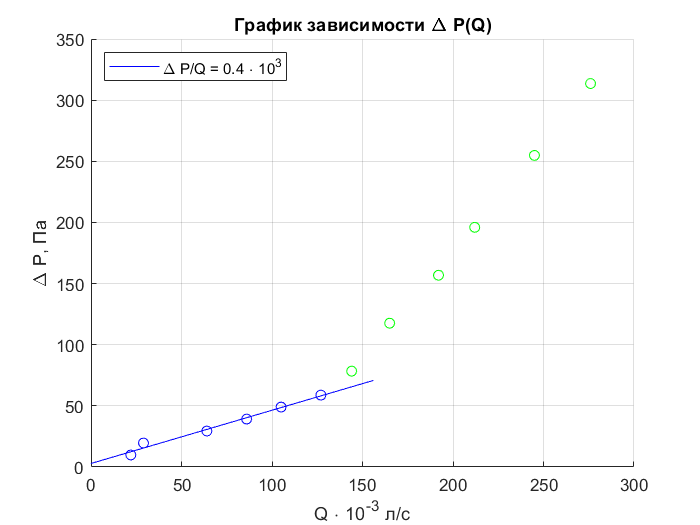
\includegraphics[width=0.9\linewidth]{plot_2.png}
\end{center}

Найдём $\eta$:

\[
\eta = \dfrac{\pi \cdot 0.00525 ^ 4}{8 \cdot 2^4 \cdot 0.5 \cdot 2.14 \cdot 10^{-6}} = 1.74 \cdot 10^{-5} \text{Па} \cdot \text{с},
\]
\[
\sigma_\eta = \eta \cdot \sqrt{4 \cdot \left( \frac{\sigma_R}{R} \right) ^ 2 + \left( \frac{\sigma_l}{l} \right) ^ 2 + \left( \frac{\sigma_b}{b} \right) ^ 2}, 
\]\[
\sigma_\eta = 1.74 \cdot 10^{-5} \cdot \sqrt{4 \cdot \left(\frac{0.05}{5.25} \right) ^ 2 + \left( \frac{0.1}{50} \right) ^ 2 + \left( \frac{0.02}{2.14} \right) ^ 2} = 0.02 \cdot 10 ^ {-5}.
\]

Получили $\eta = (1.74 \pm 0.02) \cdot 10^{-5}$ Па $\cdot$ с.
Найдём критическое число Рейнольдса при $Q = 0.13$ л/с:

\[
Re_\text{кр} = \frac{4 Q \rho}{\eta \pi d} = \frac{4 \cdot 0.13 \cdot 10^{-3} \cdot 1.2}{1.74 \cdot 10^{-5} \cdot \pi \cdot 0.00525} \approx 2200
\] 

\item Найдём зависимость $\Delta P$ от положения концов манометра на трубе.

\begin{figure}[h!]
\centering
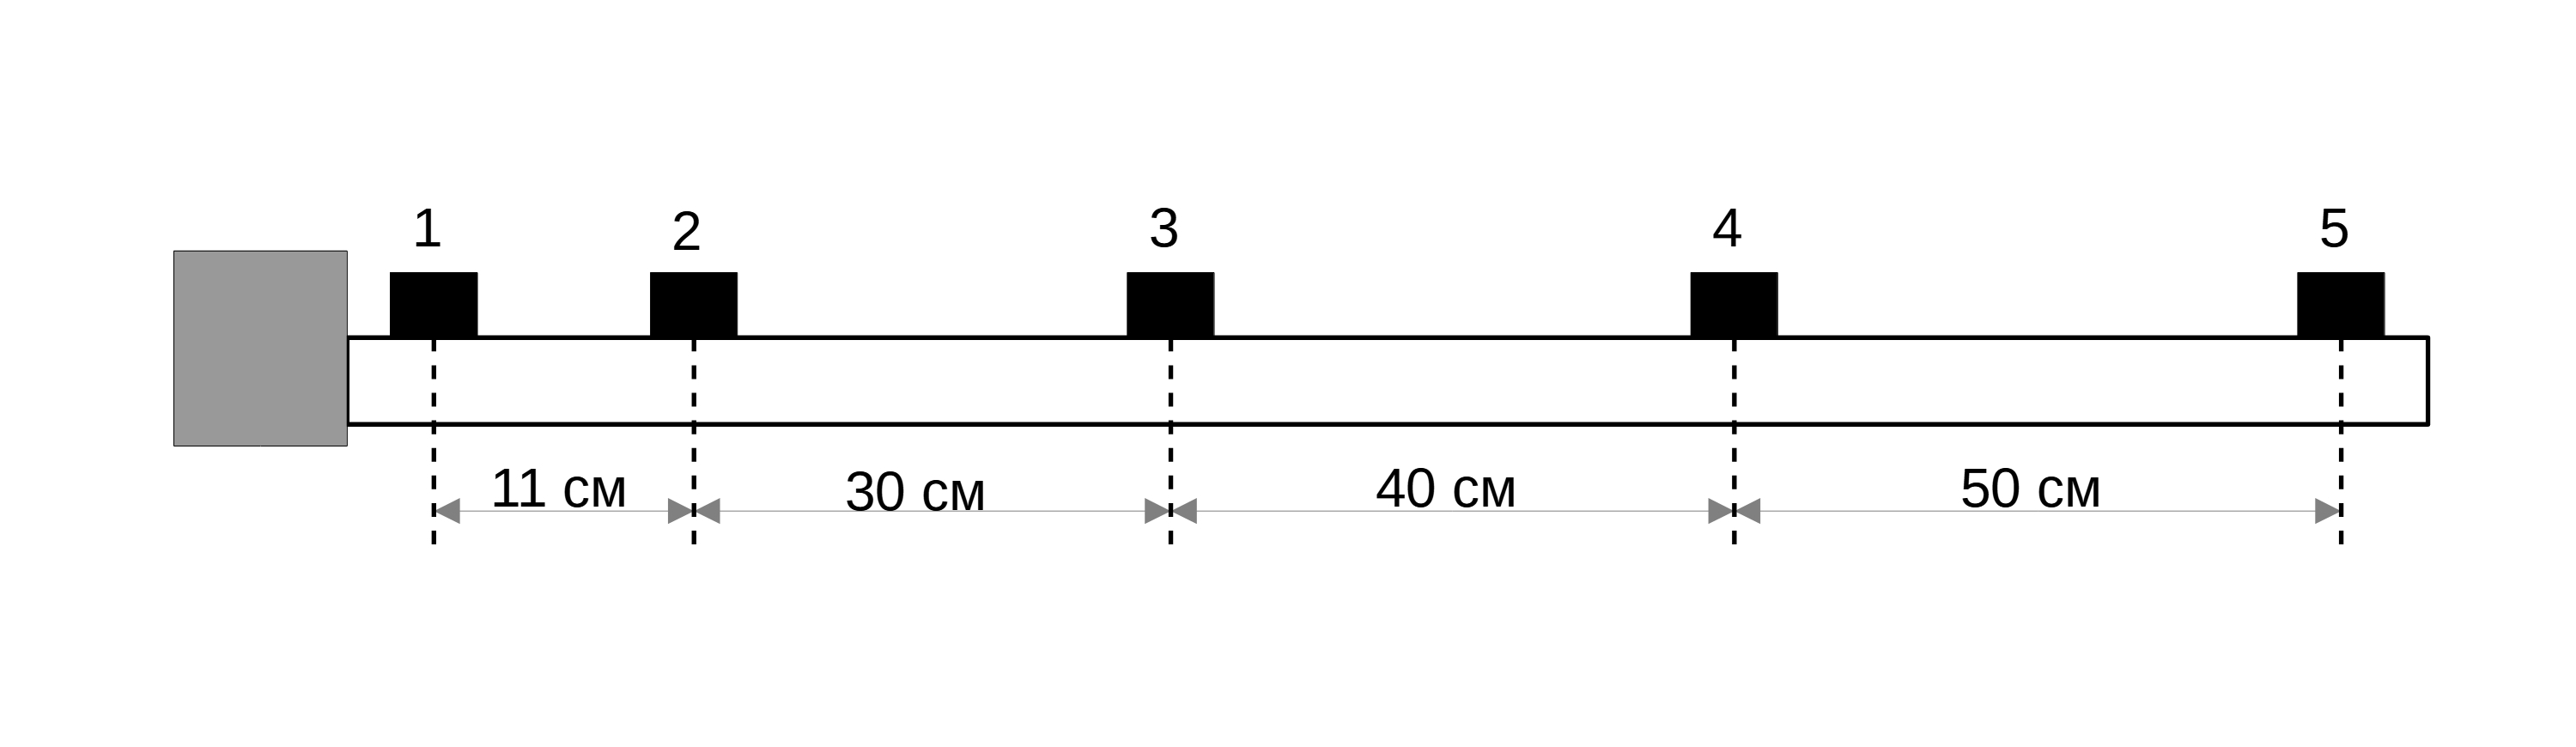
\includegraphics[width=0.8\textwidth]{setup2.jpg}
\caption{Положение разъёмов на трубе}
\label{setup2}
\end{figure}

Будем измерять перепад давления на разных участках трубы при одинаковом расходе воздуха. Для этого будем подключать концы манометра к разъёмам на трубе. Данные покажем на графике.

\begin{figure}[h!]
\centering
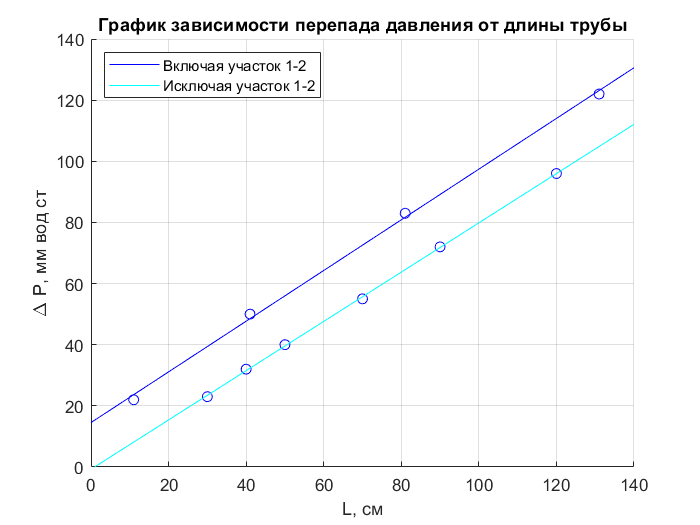
\includegraphics[width=0.8\textwidth]{plot_3.png}
\label{setup2}
\end{figure}
\end{enumerate}
\section{Выводы:}
\begin{enumerate}
\itemsep0em
\item Получили два разных значений для вязкости воздуха и $Re_\text{кр}$ при разных диаметрах труб.
\[
	\eta_1 = (2.06 \pm 0.07) \cdot 10^{-5} \; \text{Па} \cdot \text{c}, \; Re_\text{кр1} = 1700,
\]\[
	\eta_2 = (1.74 \pm 0.02) \cdot 10^{-5} \; \text{Па} \cdot \text{c}, \; Re_\text{кр2} = 2200.
\]

\item Показали линейную зависимость $\Delta P$ от длины. При этом нашли резкий перепад давления на промежутке между 1 и 2 разъёмом.
\item Убедились, что в данном случае можно использовать закон Пуазейля 
\item На последнем графике обнаружили особенность, что при включении участка, равного 11 см, давление повышается на $\approx 18$ мм вод ст. Это может быть связано с тем, что на участке 1-2 воздух не прошел длину установления потока, что увеличивает давление 

\end{enumerate}
\end{document}